\section{Iteración VI}
\subsection{Resumen}
Aquí desarrollamos una forma de gestionar proyectos dentro de la aplicación para así crear escenarios dentro de estos.

\subsection{Desarrollo}
Los escenarios generados por la aplicación están agrupados por proyectos, esto debido a que un diseñador de interiores puede realizar varias obras relacionadas entre sí, normalmente cuando son para el mismo cliente. Antes de crear escenarios, es necesario crear proyectos que los contengan y estos proyectos contienen la siguiente información del cliente:
\begin{itemize}
	\item Nombre
	\item Apellido
	\item Teléfono
	\item Email
\end{itemize}

Tras iniciar sesión se muestran los proyectos que han sido creados por el usuario (ver figura 4.39), con la opción de eliminarlos o modificar sus datos (ver figura 4.40). Asimismo el usuario puede agregar un nuevo proyecto (ver figura 4.41), el cual aparecerá en el listado de proyectos.


\begin{figure}[h!]
	\begin{minipage}{0.32\textwidth}
		\centering
		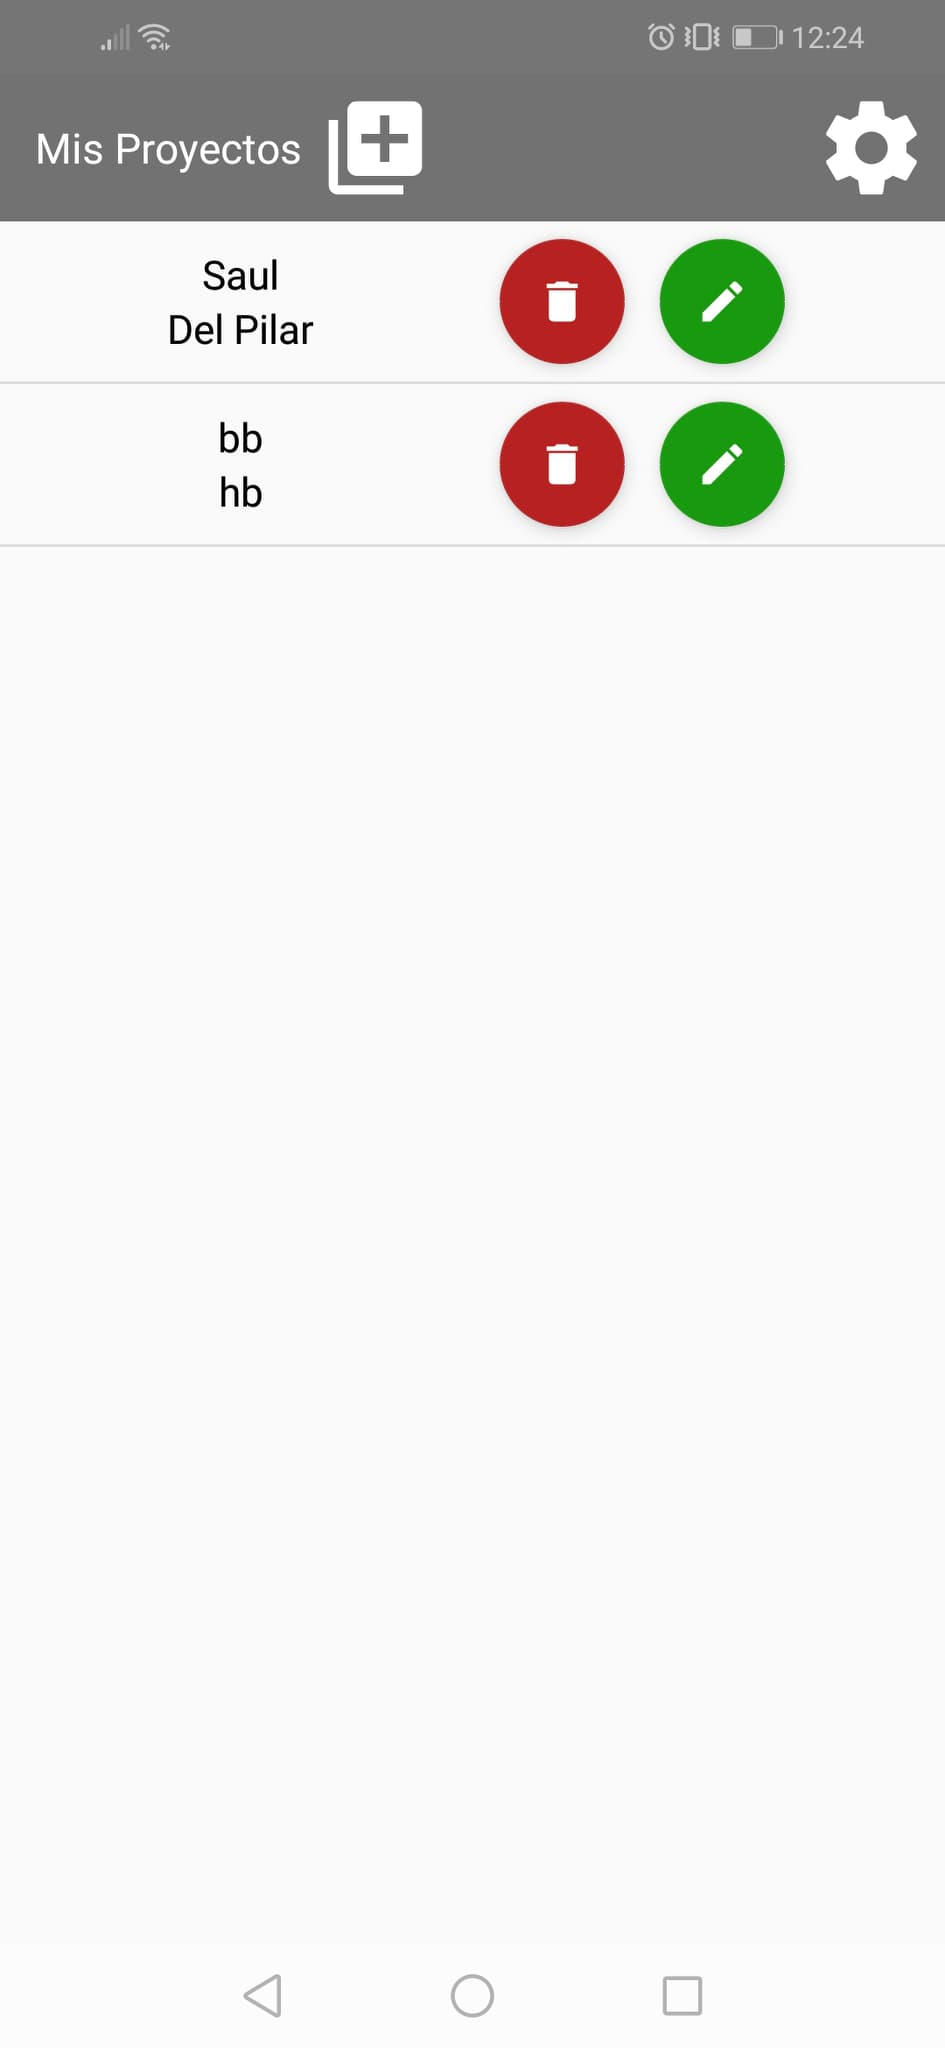
\includegraphics[width=4cm,height=8cm]{imagenes/desarrollo/app/proyectos.jpg}
		\caption{Visualización de proyectos}
		\label{fig:appreadproj}
	\end{minipage}\hfill
	\begin{minipage}{0.32\textwidth}
		\centering
		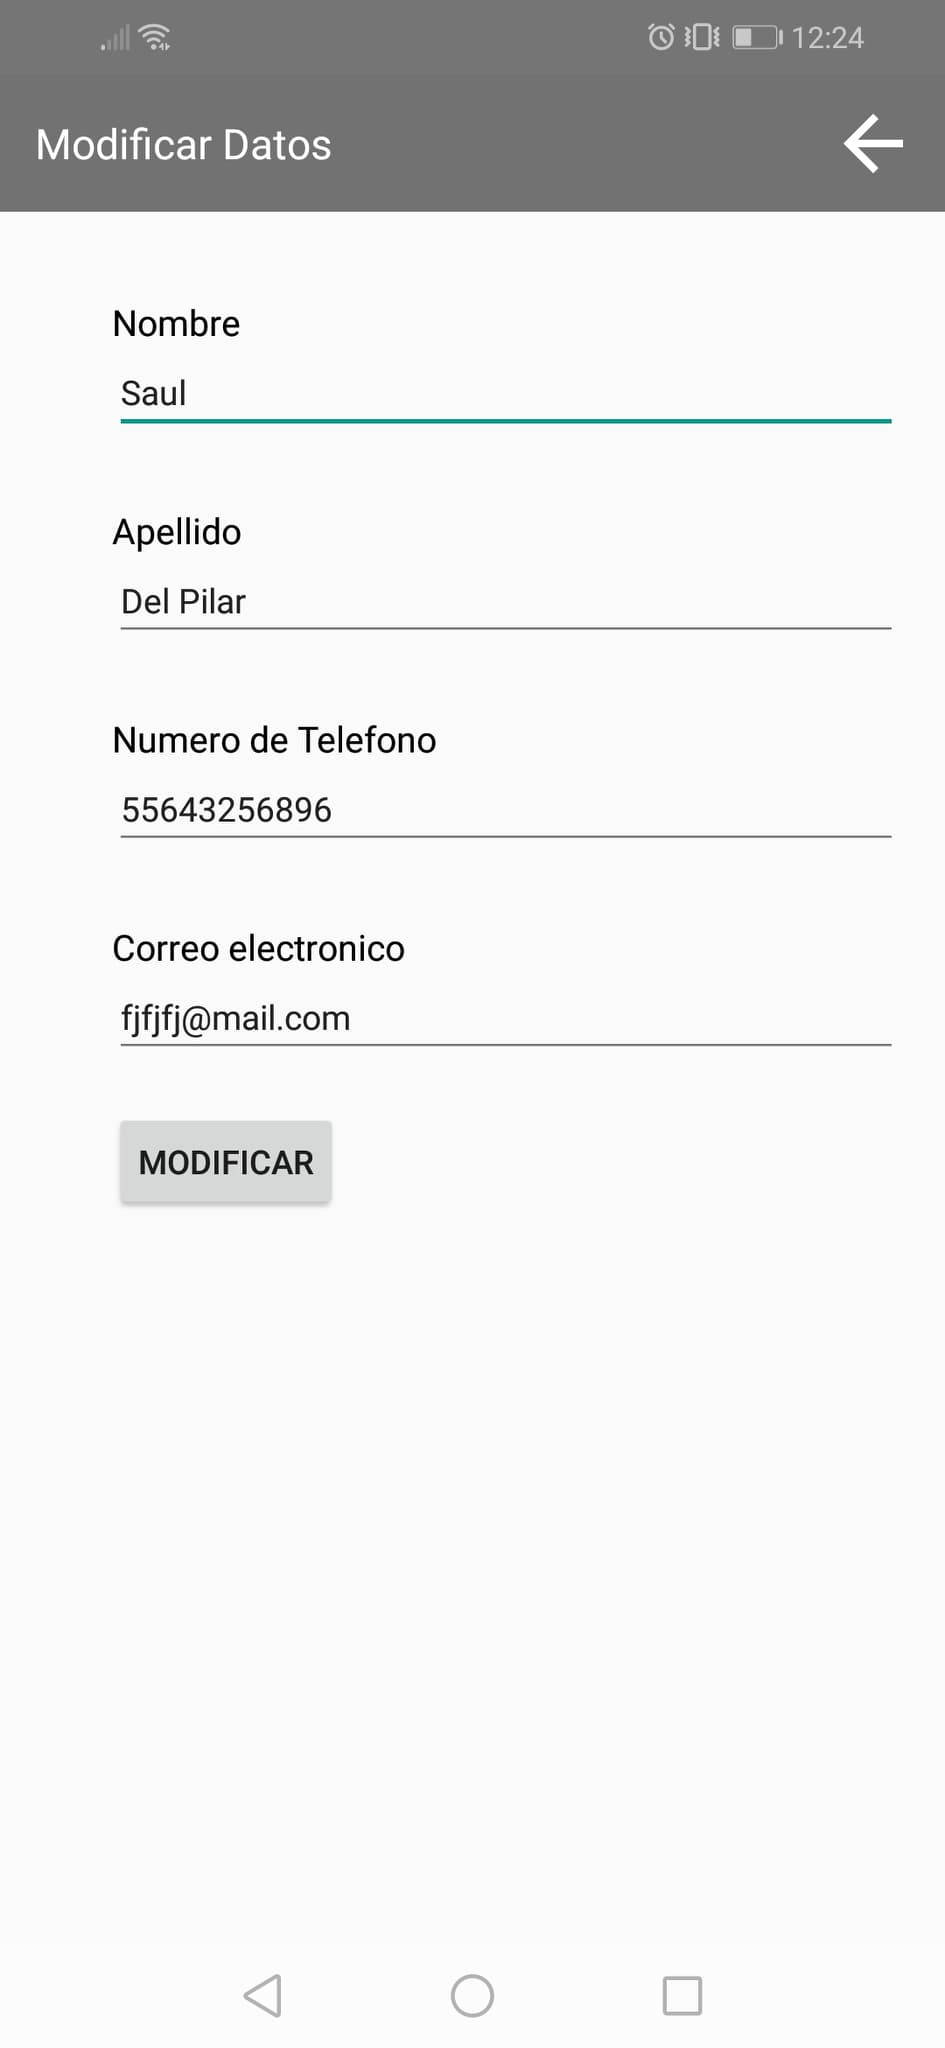
\includegraphics[width=4cm,height=8cm]{imagenes/desarrollo/app/update_proy.jpg}
		\caption{Actualización de proyecto}
		\label{fig:updateproj}
	\end{minipage}\hfill
	\begin{minipage}{0.32\textwidth}
		\centering
		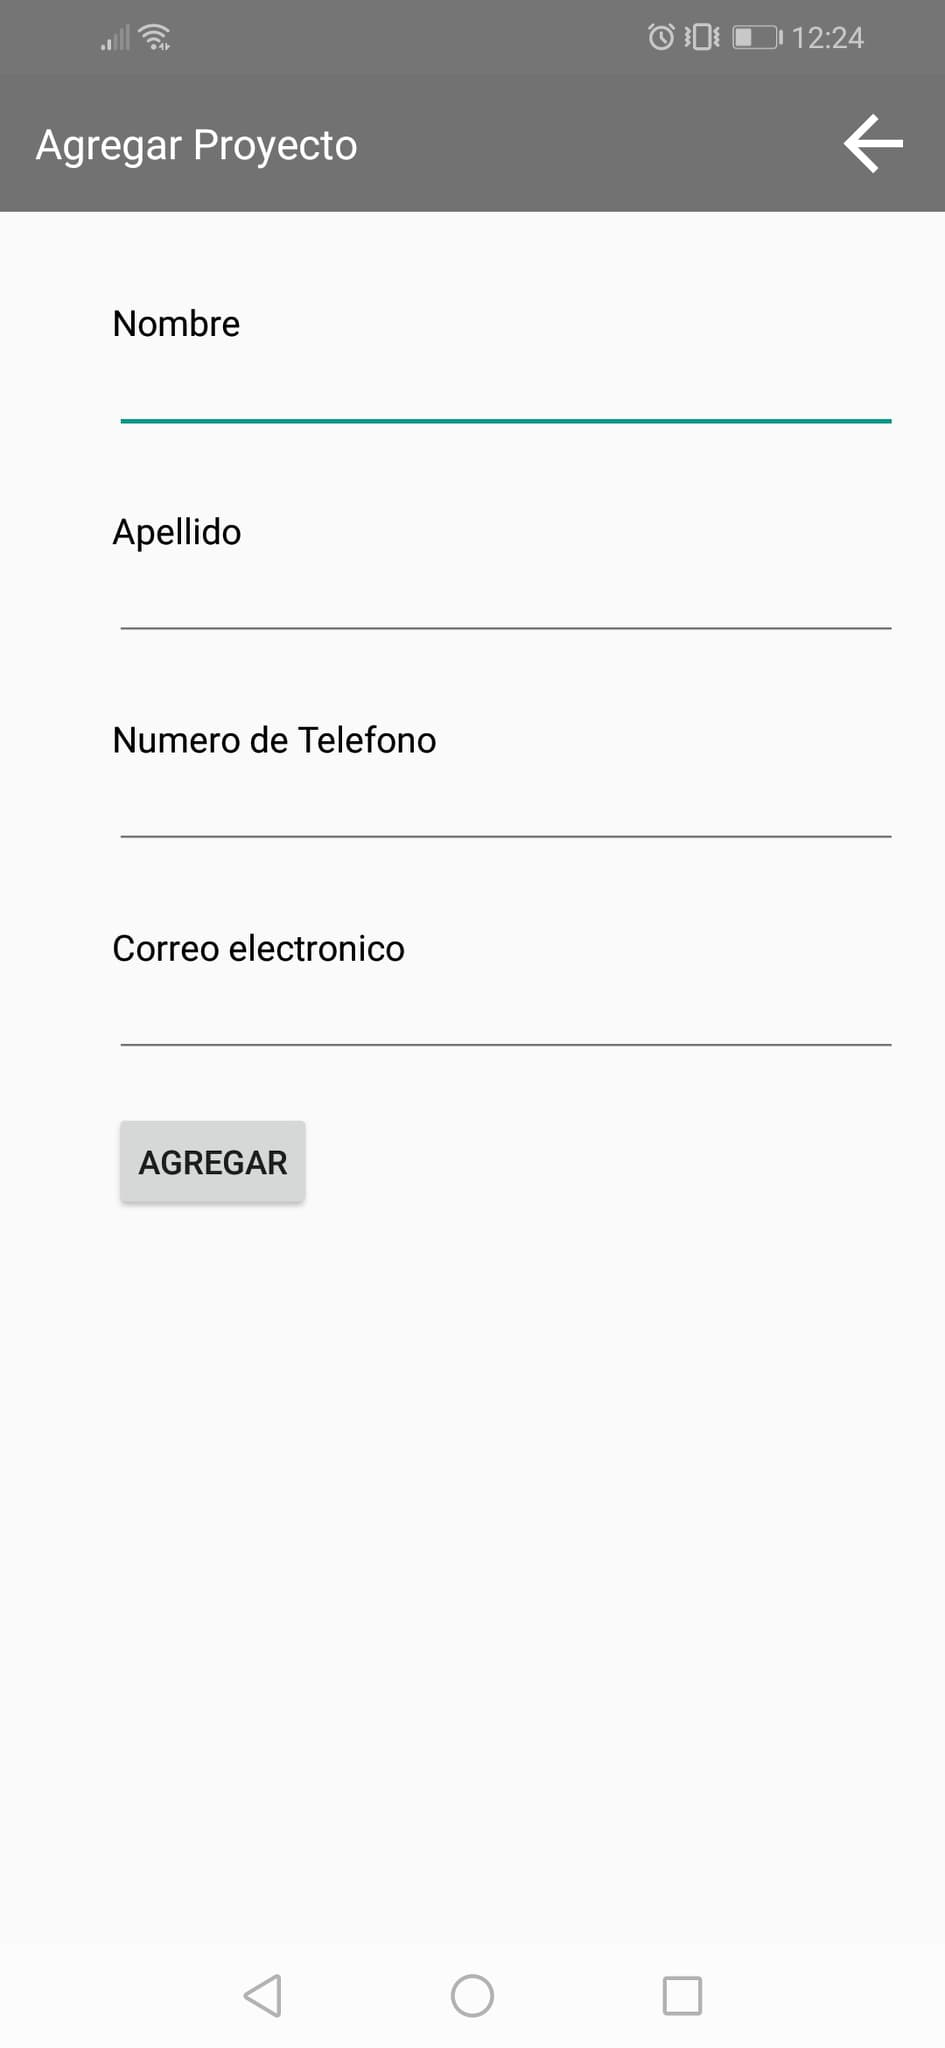
\includegraphics[width=4cm,height=8cm]{imagenes/desarrollo/app/add_proy.jpg}
		\caption{Agregar nuevo proyecto}
		\label{fig:addproj}
	\end{minipage}\hfill
\end{figure}

Esta funcionalidad cumple cuatro procesos de negocios, correspondientes a las funciones de creación, lectura, actualización y eliminación de proyectos (ver figuras 4.42, 4.43, 4.44 y 4.45)
\clearpage
\begin{figure}[h!]
	\centering
	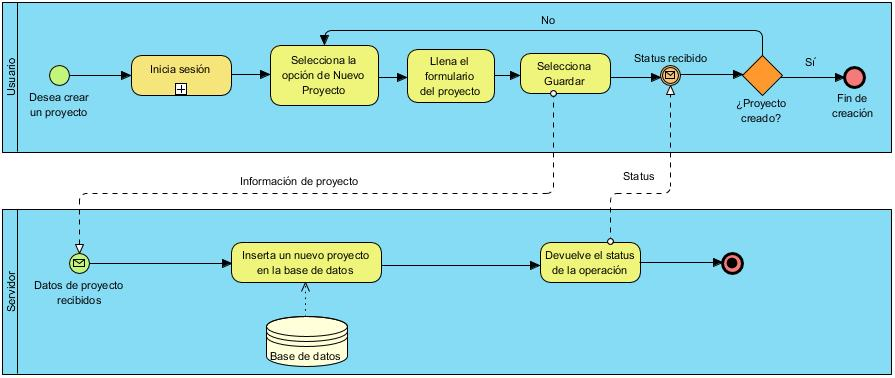
\includegraphics[width=15cm,height=7cm]{imagenes/desarrollo/diagramas/BPMN_CREATE_PROJECT.jpg}
	\caption{Diagrama de proceso de creación de proyecto.}
	\label{fig:createproject}
\end{figure}
\begin{figure}[h!]
	\centering
	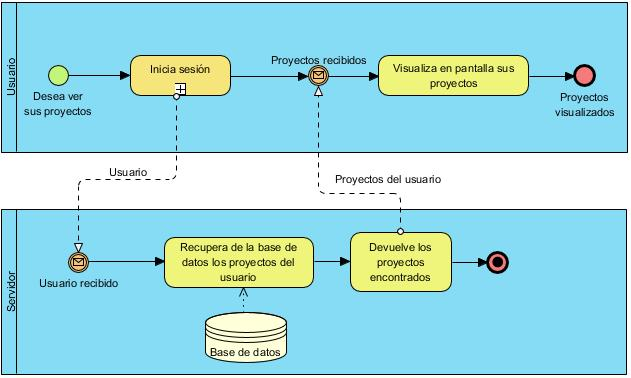
\includegraphics[width=15cm,height=9cm]{imagenes/desarrollo/diagramas/BPMN_READ_PROJECTS.jpg}
	\caption{Diagrama de proceso de lectura de proyectos.}
	\label{fig:readproject}
\end{figure}
\begin{figure}[h!]
	\centering
	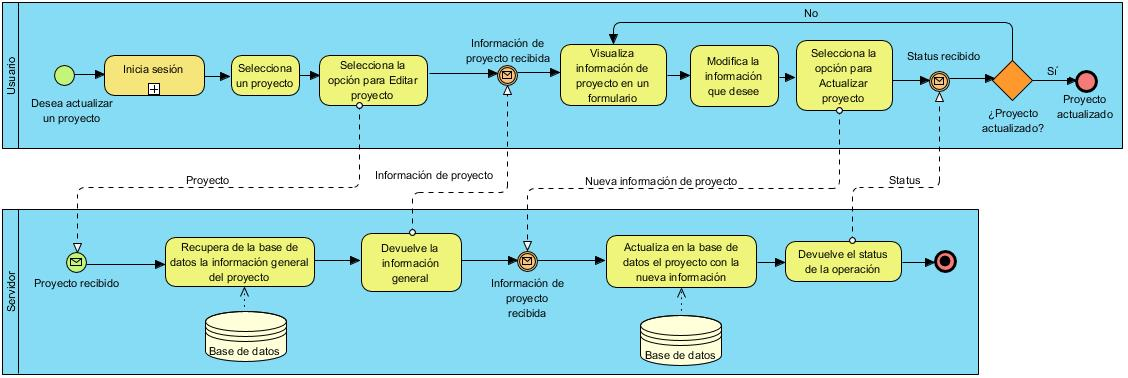
\includegraphics[width=17cm,height=6.5cm]{imagenes/desarrollo/diagramas/BPMN_UPDATE_PROJECT.jpg}
	\caption{Diagrama de proceso de actualización de proyecto.}
	\label{fig:updateproject}
\end{figure}
\begin{figure}[h!]
	\centering
	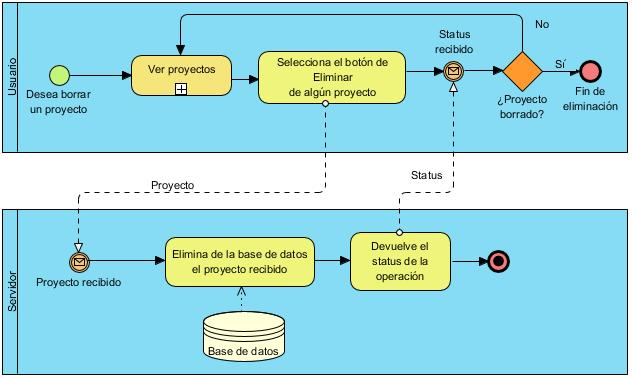
\includegraphics[width=15cm,height=9cm]{imagenes/desarrollo/diagramas/BPMN_DELETE_PROJECT.jpg}
	\caption{Diagrama de proceso de eliminación de proyecto.}
	\label{fig:deleteproject}
\end{figure}
\clearpage